\documentclass[a4paper,pdftex,12pt]{article} % A4 paper and 11pt font size

\usepackage[T1]{fontenc} % Use 8-bit encoding that has 256 glyphs
\usepackage[english,slovene]{babel} % English language/hyphenation

\usepackage{amsmath,amsfonts,amsthm,amssymb,mathrsfs} % Math packages
\usepackage{mathtools}
\usepackage{dsfont}

\usepackage[gen]{eurosym} %Euro


\usepackage[pdftex]{graphicx}

\usepackage{sectsty} % Allows customizing section commands
%\allsectionsfont{\centering \normalfont\scshape} % Make all sections centered, the default font and small caps
\renewcommand{\vec}[1]{\boldsymbol{\mathbf{#1}}}                                        
\newcommand{\ihat}[0]{\boldsymbol{\mathbf{\oldhat{\textbf{\i}}}}} % pokončna j in i (j i n i

\usepackage{fancyhdr} % Custom headers and footers
\pagestyle{fancyplain} % Makes all pages in the document conform to the custom headers and footers
\fancyhead{} % No page header - if you want one, create it in the same way as the footers below
\fancyfoot[L]{} % Empty left footer
\fancyfoot[C]{} % Empty center footer
\fancyfoot[R]{\thepage} % Page numbering for right footer
\renewcommand{\headrulewidth}{0pt} % Remove header underlines
\renewcommand{\footrulewidth}{0pt} % Remove footer underlines
\setlength{\headheight}{13.6pt} % Customize the height of the header

\numberwithin{equation}{section} % Number equations within sections (i.e. 1.1, 1.2, 2.1, 2.2 instead of 1, 2, 3, 4)
\numberwithin{figure}{section} % Number figures within sections (i.e. 1.1, 1.2, 2.1, 2.2 instead of 1, 2, 3, 4)
\numberwithin{table}{section} % Number tables within sections (i.e. 1.1, 1.2, 2.1, 2.2 instead of 1, 2, 3, 4)

\setlength\parindent{0pt} % Removes all indentation from paragraphs - comment this line for an assignment with lots of text

%----------------------------------------------------------------------------------------
%	TITLE SECTION
%----------------------------------------------------------------------------------------

\newcommand{\horrule}[1]{\rule{\linewidth}{#1}} % Create horizontal rule command with 1 argument of height

\title{	
\normalfont \normalsize 
\textsc{Modelska analiza 1} \\ [25pt] % Your university, school and/or department name(s)
%\horrule{0.2pt} \\[0.4cm] % Thin top horizontal rule
\huge 2. naloga\\ % The assignment title
%\horrule{0.2pt} \\[0.5cm] % Thick bottom horizontal rule
}

\author{Tina Klobas} % Your name

\date{\normalsize\today} % Today's date or a custom date

\begin{document}

\maketitle % Print the title

\section{Opis problema}
Želimo sestaviti tak jedilnik iz nabora danih živil, da bomo dnevno zaužili minimalno 
kalorij, hkrati pa zadostili priporočilom za dnevne vnose različnih hranilnih snovi. 
Te naloge se lotimo kot vsakega linearnega programiranja, kjer iščemo optimum linearne 
funkcije (kriterijska funkcija), v~našem primeru kalorije, pri danih omejitvah. Zapišimo
to s~sistemom linearnih enačb:
\begin{eqnarray*} 
    \mathrm{kalorije} &=& x_1 c_1 + x_2 c_1 + \cdots + x_n c_n = \mathrm{min} \\
	b_1 &=& x_1 a_{11} + x_2 a_{12} + \cdots + x_n a_{1n} \\
	b_2 &=& x_1 a_{21} + x_2 a_{22} + \cdots + x_n a_{2n} \\
	b_3 &=& x_1 a_{31} + x_2 a_{32} + \cdots + x_n a_{3n} \\
	    &\vdots& \\ 
	b_n &=& x_1 a_{n1} + x_2 a_{n2} + \cdots + x_n a_{nn}.
\end{eqnarray*}
Iščemo torej:
\begin{align}\label{matrika}
    \text{min } &\vec{c}^T \vec{x}  \\
    \text{pri omejitvah } &A \vec{x} \geq \vec{b}, 
\end{align}
kjer je $A$ matrika koeficientov $a_{ij}$, $\vec{b}$ vektor prostih členov, $\vec{c}$ vektor
koeficientov kriterijske funkcije, $\vec{x}$ pa vektor spremenljivk. Za grafični prikaz
problema vsako količino, ki jo zapišemo v~stolpce matrike $A$ prikažemo na svoji osi
in potem z~linearnimi enačbami omejujemo naš prostor rešitve. Minimum tako nastopa v~enem
od oglišč večkotnika v~n-dimenzijah.

%----------------------------------------------------------------------------------------
%	PROBLEM 1
%----------------------------------------------------------------------------------------

\section{Minimizacija kalorij}
Za začetek si poglejmo primer, ko minimiziramo količino kalorij pri priporočenih dnevnih
vnosih:
\begin{itemize}\label{tabela1}
    \item[--]$70$g maščob,
    \item[--]$310$g ogljikovih hidratov,
    \item[--]$50$g proteinov,
    \item[--]$1000$mg kalcija in
    \item[--]$18$mg železa.
\end{itemize}
\begin{figure}    
    % GNUPLOT: LaTeX picture with Postscript
\begingroup
  \makeatletter
  \providecommand\color[2][]{%
    \GenericError{(gnuplot) \space\space\space\@spaces}{%
      Package color not loaded in conjunction with
      terminal option `colourtext'%
    }{See the gnuplot documentation for explanation.%
    }{Either use 'blacktext' in gnuplot or load the package
      color.sty in LaTeX.}%
    \renewcommand\color[2][]{}%
  }%
  \providecommand\includegraphics[2][]{%
    \GenericError{(gnuplot) \space\space\space\@spaces}{%
      Package graphicx or graphics not loaded%
    }{See the gnuplot documentation for explanation.%
    }{The gnuplot epslatex terminal needs graphicx.sty or graphics.sty.}%
    \renewcommand\includegraphics[2][]{}%
  }%
  \providecommand\rotatebox[2]{#2}%
  \@ifundefined{ifGPcolor}{%
    \newif\ifGPcolor
    \GPcolortrue
  }{}%
  \@ifundefined{ifGPblacktext}{%
    \newif\ifGPblacktext
    \GPblacktexttrue
  }{}%
  % define a \g@addto@macro without @ in the name:
  \let\gplgaddtomacro\g@addto@macro
  % define empty templates for all commands taking text:
  \gdef\gplbacktext{}%
  \gdef\gplfronttext{}%
  \makeatother
  \ifGPblacktext
    % no textcolor at all
    \def\colorrgb#1{}%
    \def\colorgray#1{}%
  \else
    % gray or color?
    \ifGPcolor
      \def\colorrgb#1{\color[rgb]{#1}}%
      \def\colorgray#1{\color[gray]{#1}}%
      \expandafter\def\csname LTw\endcsname{\color{white}}%
      \expandafter\def\csname LTb\endcsname{\color{black}}%
      \expandafter\def\csname LTa\endcsname{\color{black}}%
      \expandafter\def\csname LT0\endcsname{\color[rgb]{1,0,0}}%
      \expandafter\def\csname LT1\endcsname{\color[rgb]{0,1,0}}%
      \expandafter\def\csname LT2\endcsname{\color[rgb]{0,0,1}}%
      \expandafter\def\csname LT3\endcsname{\color[rgb]{1,0,1}}%
      \expandafter\def\csname LT4\endcsname{\color[rgb]{0,1,1}}%
      \expandafter\def\csname LT5\endcsname{\color[rgb]{1,1,0}}%
      \expandafter\def\csname LT6\endcsname{\color[rgb]{0,0,0}}%
      \expandafter\def\csname LT7\endcsname{\color[rgb]{1,0.3,0}}%
      \expandafter\def\csname LT8\endcsname{\color[rgb]{0.5,0.5,0.5}}%
    \else
      % gray
      \def\colorrgb#1{\color{black}}%
      \def\colorgray#1{\color[gray]{#1}}%
      \expandafter\def\csname LTw\endcsname{\color{white}}%
      \expandafter\def\csname LTb\endcsname{\color{black}}%
      \expandafter\def\csname LTa\endcsname{\color{black}}%
      \expandafter\def\csname LT0\endcsname{\color{black}}%
      \expandafter\def\csname LT1\endcsname{\color{black}}%
      \expandafter\def\csname LT2\endcsname{\color{black}}%
      \expandafter\def\csname LT3\endcsname{\color{black}}%
      \expandafter\def\csname LT4\endcsname{\color{black}}%
      \expandafter\def\csname LT5\endcsname{\color{black}}%
      \expandafter\def\csname LT6\endcsname{\color{black}}%
      \expandafter\def\csname LT7\endcsname{\color{black}}%
      \expandafter\def\csname LT8\endcsname{\color{black}}%
    \fi
  \fi
    \setlength{\unitlength}{0.0500bp}%
    \ifx\gptboxheight\undefined%
      \newlength{\gptboxheight}%
      \newlength{\gptboxwidth}%
      \newsavebox{\gptboxtext}%
    \fi%
    \setlength{\fboxrule}{0.5pt}%
    \setlength{\fboxsep}{1pt}%
\begin{picture}(7200.00,4320.00)%
    \gplgaddtomacro\gplbacktext{%
      \csname LTb\endcsname%%
      \put(459,186){\makebox(0,0)[r]{\strut{}$-18$}}%
      \csname LTb\endcsname%%
      \put(459,813){\makebox(0,0)[r]{\strut{}$-15$}}%
      \csname LTb\endcsname%%
      \put(459,1440){\makebox(0,0)[r]{\strut{}$-12$}}%
      \csname LTb\endcsname%%
      \put(459,2067){\makebox(0,0)[r]{\strut{}$-9$}}%
      \csname LTb\endcsname%%
      \put(459,2693){\makebox(0,0)[r]{\strut{}$-6$}}%
      \csname LTb\endcsname%%
      \put(459,3320){\makebox(0,0)[r]{\strut{}$-3$}}%
      \csname LTb\endcsname%%
      \put(459,3947){\makebox(0,0)[r]{\strut{}$0$}}%
      \csname LTb\endcsname%%
      \put(561,4133){\makebox(0,0){\strut{}$0$}}%
      \csname LTb\endcsname%%
      \put(2144,4133){\makebox(0,0){\strut{}$4$}}%
      \csname LTb\endcsname%%
      \put(3727,4133){\makebox(0,0){\strut{}$8$}}%
      \csname LTb\endcsname%%
      \put(5310,4133){\makebox(0,0){\strut{}$12$}}%
      \csname LTb\endcsname%%
      \put(6893,4133){\makebox(0,0){\strut{}$16$}}%
    }%
    \gplgaddtomacro\gplfronttext{%
      \csname LTb\endcsname%%
      \put(2489,3390){\makebox(0,0)[l]{\strut{}diskretni nivoji (sosedi)}}%
      \csname LTb\endcsname%%
      \put(2489,3576){\makebox(0,0)[l]{\strut{}diskretni nivoji (poljubni)}}%
      \csname LTb\endcsname%%
      \put(2489,3762){\makebox(0,0)[l]{\strut{}zvezni nivoji}}%
    }%
    \gplbacktext
    \put(0,0){\includegraphics{graf1}}%
    \gplfronttext
  \end{picture}%
\endgroup

    \caption{Prikaz dnevne prehrane, ko upoštevamo le del priporočenih dnevnih vnosov 
    snovi.}
    \label{graf1}
\end{figure}

Problem preoblikujemo v~matrični sistem~\ref{matrika}, kjer v~matriko $A$ ustavimo količine 
iz tabele podatkov za hranilne vrednosti živil, v~vektor $\vec{b}$ priporočene dnevne 
količine hranilnih snovi v~$\vec{c}$ pa vstavimo kalorije vseh živil. Da upoštevamo še
dodaten pogoj, da na dan ne pojemo več kot dva kilograma hrane, v~matriko $A$ vstavimo
vrstico minus enk, v~$\vec{b}$ pa $2kg$. Vse skupaj še normiramo na $100$g hrane, kar
saj so vse količine v~tabeli podane za $100$g hrane. Tako dobimo priporočen dnevni jedilnik
prikazan na diagramu~\ref{graf1}. Seveda tega v~praksi noben dietetik ne bi predpisal take 
prehrane, in tudi z~dodatnimi pogoji
\begin{itemize}
    \item[--]$60$mg vitamina C,
    \item[--]$3500$mg kalija ter
    \item[--]$500$mg -- $2400$mg natrija.
\end{itemize}
raznovrstnosti jedilnika ne izboljšamo, kar je vidno tudi na sliki~\ref{graf2}.
\begin{figure}    
    % GNUPLOT: LaTeX picture with Postscript
\begingroup
  \makeatletter
  \providecommand\color[2][]{%
    \GenericError{(gnuplot) \space\space\space\@spaces}{%
      Package color not loaded in conjunction with
      terminal option `colourtext'%
    }{See the gnuplot documentation for explanation.%
    }{Either use 'blacktext' in gnuplot or load the package
      color.sty in LaTeX.}%
    \renewcommand\color[2][]{}%
  }%
  \providecommand\includegraphics[2][]{%
    \GenericError{(gnuplot) \space\space\space\@spaces}{%
      Package graphicx or graphics not loaded%
    }{See the gnuplot documentation for explanation.%
    }{The gnuplot epslatex terminal needs graphicx.sty or graphics.sty.}%
    \renewcommand\includegraphics[2][]{}%
  }%
  \providecommand\rotatebox[2]{#2}%
  \@ifundefined{ifGPcolor}{%
    \newif\ifGPcolor
    \GPcolortrue
  }{}%
  \@ifundefined{ifGPblacktext}{%
    \newif\ifGPblacktext
    \GPblacktexttrue
  }{}%
  % define a \g@addto@macro without @ in the name:
  \let\gplgaddtomacro\g@addto@macro
  % define empty templates for all commands taking text:
  \gdef\gplbacktext{}%
  \gdef\gplfronttext{}%
  \makeatother
  \ifGPblacktext
    % no textcolor at all
    \def\colorrgb#1{}%
    \def\colorgray#1{}%
  \else
    % gray or color?
    \ifGPcolor
      \def\colorrgb#1{\color[rgb]{#1}}%
      \def\colorgray#1{\color[gray]{#1}}%
      \expandafter\def\csname LTw\endcsname{\color{white}}%
      \expandafter\def\csname LTb\endcsname{\color{black}}%
      \expandafter\def\csname LTa\endcsname{\color{black}}%
      \expandafter\def\csname LT0\endcsname{\color[rgb]{1,0,0}}%
      \expandafter\def\csname LT1\endcsname{\color[rgb]{0,1,0}}%
      \expandafter\def\csname LT2\endcsname{\color[rgb]{0,0,1}}%
      \expandafter\def\csname LT3\endcsname{\color[rgb]{1,0,1}}%
      \expandafter\def\csname LT4\endcsname{\color[rgb]{0,1,1}}%
      \expandafter\def\csname LT5\endcsname{\color[rgb]{1,1,0}}%
      \expandafter\def\csname LT6\endcsname{\color[rgb]{0,0,0}}%
      \expandafter\def\csname LT7\endcsname{\color[rgb]{1,0.3,0}}%
      \expandafter\def\csname LT8\endcsname{\color[rgb]{0.5,0.5,0.5}}%
    \else
      % gray
      \def\colorrgb#1{\color{black}}%
      \def\colorgray#1{\color[gray]{#1}}%
      \expandafter\def\csname LTw\endcsname{\color{white}}%
      \expandafter\def\csname LTb\endcsname{\color{black}}%
      \expandafter\def\csname LTa\endcsname{\color{black}}%
      \expandafter\def\csname LT0\endcsname{\color{black}}%
      \expandafter\def\csname LT1\endcsname{\color{black}}%
      \expandafter\def\csname LT2\endcsname{\color{black}}%
      \expandafter\def\csname LT3\endcsname{\color{black}}%
      \expandafter\def\csname LT4\endcsname{\color{black}}%
      \expandafter\def\csname LT5\endcsname{\color{black}}%
      \expandafter\def\csname LT6\endcsname{\color{black}}%
      \expandafter\def\csname LT7\endcsname{\color{black}}%
      \expandafter\def\csname LT8\endcsname{\color{black}}%
    \fi
  \fi
    \setlength{\unitlength}{0.0500bp}%
    \ifx\gptboxheight\undefined%
      \newlength{\gptboxheight}%
      \newlength{\gptboxwidth}%
      \newsavebox{\gptboxtext}%
    \fi%
    \setlength{\fboxrule}{0.5pt}%
    \setlength{\fboxsep}{1pt}%
\begin{picture}(7200.00,5040.00)%
    \gplgaddtomacro\gplbacktext{%
      \csname LTb\endcsname%%
      \put(946,2350){\makebox(0,0)[r]{\strut{}$1$}}%
      \put(946,704){\makebox(0,0)[r]{\strut{}$10^{-4}$}}%
      \put(946,1527){\makebox(0,0)[r]{\strut{}$10^{-2}$}}%
      \put(946,3173){\makebox(0,0)[r]{\strut{}$10^{2}$}}%
      \put(946,3996){\makebox(0,0)[r]{\strut{}$10^{4}$}}%
      \put(946,4819){\makebox(0,0)[r]{\strut{}$10^{6}$}}%
      \put(1078,484){\makebox(0,0){\strut{}$0$}}%
      \put(2223,484){\makebox(0,0){\strut{}$0.1$}}%
      \put(3368,484){\makebox(0,0){\strut{}$0.2$}}%
      \put(4513,484){\makebox(0,0){\strut{}$0.3$}}%
      \put(5658,484){\makebox(0,0){\strut{}$0.4$}}%
      \put(6803,484){\makebox(0,0){\strut{}$0.5$}}%
    }%
    \gplgaddtomacro\gplfronttext{%
      \csname LTb\endcsname%%
      \put(209,2761){\rotatebox{-270}{\makebox(0,0){\strut{}$|f|^2$}}}%
      \put(3940,154){\makebox(0,0){\strut{}$\omega$}}%
      \csname LTb\endcsname%%
      \put(1669,4404){\makebox(0,0)[l]{\strut{}val2}}%
      \csname LTb\endcsname%%
      \put(1669,4624){\makebox(0,0)[l]{\strut{}val3}}%
    }%
    \gplbacktext
    \put(0,0){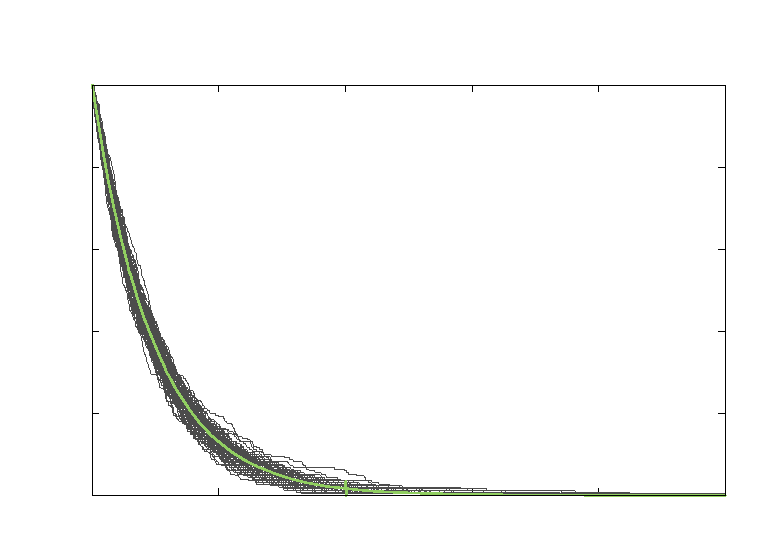
\includegraphics[width={360.00bp},height={252.00bp}]{graf2}}%
    \gplfronttext
  \end{picture}%
\endgroup

    \caption{Prikaz dnevne prehrane, ko upoštevamo še drugi del priporočenih dnevnih vnosov 
    snovi.}
    \label{graf2}
\end{figure}
Povečanje raznolikosti jedilnika poskusimo doseči z~omejitvijo količine 
posameznega živila, kar upoštevamo pri oblikovanju jedilnika, ki je zaradi lažje predstave
prikazan na tortnem diagramu~\ref{graf3}.
\begin{figure}    
    % GNUPLOT: LaTeX picture with Postscript
\begingroup
  \makeatletter
  \providecommand\color[2][]{%
    \GenericError{(gnuplot) \space\space\space\@spaces}{%
      Package color not loaded in conjunction with
      terminal option `colourtext'%
    }{See the gnuplot documentation for explanation.%
    }{Either use 'blacktext' in gnuplot or load the package
      color.sty in LaTeX.}%
    \renewcommand\color[2][]{}%
  }%
  \providecommand\includegraphics[2][]{%
    \GenericError{(gnuplot) \space\space\space\@spaces}{%
      Package graphicx or graphics not loaded%
    }{See the gnuplot documentation for explanation.%
    }{The gnuplot epslatex terminal needs graphicx.sty or graphics.sty.}%
    \renewcommand\includegraphics[2][]{}%
  }%
  \providecommand\rotatebox[2]{#2}%
  \@ifundefined{ifGPcolor}{%
    \newif\ifGPcolor
    \GPcolortrue
  }{}%
  \@ifundefined{ifGPblacktext}{%
    \newif\ifGPblacktext
    \GPblacktexttrue
  }{}%
  % define a \g@addto@macro without @ in the name:
  \let\gplgaddtomacro\g@addto@macro
  % define empty templates for all commands taking text:
  \gdef\gplbacktext{}%
  \gdef\gplfronttext{}%
  \makeatother
  \ifGPblacktext
    % no textcolor at all
    \def\colorrgb#1{}%
    \def\colorgray#1{}%
  \else
    % gray or color?
    \ifGPcolor
      \def\colorrgb#1{\color[rgb]{#1}}%
      \def\colorgray#1{\color[gray]{#1}}%
      \expandafter\def\csname LTw\endcsname{\color{white}}%
      \expandafter\def\csname LTb\endcsname{\color{black}}%
      \expandafter\def\csname LTa\endcsname{\color{black}}%
      \expandafter\def\csname LT0\endcsname{\color[rgb]{1,0,0}}%
      \expandafter\def\csname LT1\endcsname{\color[rgb]{0,1,0}}%
      \expandafter\def\csname LT2\endcsname{\color[rgb]{0,0,1}}%
      \expandafter\def\csname LT3\endcsname{\color[rgb]{1,0,1}}%
      \expandafter\def\csname LT4\endcsname{\color[rgb]{0,1,1}}%
      \expandafter\def\csname LT5\endcsname{\color[rgb]{1,1,0}}%
      \expandafter\def\csname LT6\endcsname{\color[rgb]{0,0,0}}%
      \expandafter\def\csname LT7\endcsname{\color[rgb]{1,0.3,0}}%
      \expandafter\def\csname LT8\endcsname{\color[rgb]{0.5,0.5,0.5}}%
    \else
      % gray
      \def\colorrgb#1{\color{black}}%
      \def\colorgray#1{\color[gray]{#1}}%
      \expandafter\def\csname LTw\endcsname{\color{white}}%
      \expandafter\def\csname LTb\endcsname{\color{black}}%
      \expandafter\def\csname LTa\endcsname{\color{black}}%
      \expandafter\def\csname LT0\endcsname{\color{black}}%
      \expandafter\def\csname LT1\endcsname{\color{black}}%
      \expandafter\def\csname LT2\endcsname{\color{black}}%
      \expandafter\def\csname LT3\endcsname{\color{black}}%
      \expandafter\def\csname LT4\endcsname{\color{black}}%
      \expandafter\def\csname LT5\endcsname{\color{black}}%
      \expandafter\def\csname LT6\endcsname{\color{black}}%
      \expandafter\def\csname LT7\endcsname{\color{black}}%
      \expandafter\def\csname LT8\endcsname{\color{black}}%
    \fi
  \fi
    \setlength{\unitlength}{0.0500bp}%
    \ifx\gptboxheight\undefined%
      \newlength{\gptboxheight}%
      \newlength{\gptboxwidth}%
      \newsavebox{\gptboxtext}%
    \fi%
    \setlength{\fboxrule}{0.5pt}%
    \setlength{\fboxsep}{1pt}%
\begin{picture}(7200.00,5040.00)%
    \gplgaddtomacro\gplbacktext{%
      \csname LTb\endcsname%%
      \put(594,220){\makebox(0,0)[r]{\strut{}$-18$}}%
      \csname LTb\endcsname%%
      \put(594,950){\makebox(0,0)[r]{\strut{}$-15$}}%
      \csname LTb\endcsname%%
      \put(594,1680){\makebox(0,0)[r]{\strut{}$-12$}}%
      \csname LTb\endcsname%%
      \put(594,2410){\makebox(0,0)[r]{\strut{}$-9$}}%
      \csname LTb\endcsname%%
      \put(594,3139){\makebox(0,0)[r]{\strut{}$-6$}}%
      \csname LTb\endcsname%%
      \put(594,3869){\makebox(0,0)[r]{\strut{}$-3$}}%
      \csname LTb\endcsname%%
      \put(594,4599){\makebox(0,0)[r]{\strut{}$0$}}%
      \csname LTb\endcsname%%
      \put(726,0){\makebox(0,0){\strut{}}}%
      \csname LTb\endcsname%%
      \put(2245,0){\makebox(0,0){\strut{}}}%
      \csname LTb\endcsname%%
      \put(3765,0){\makebox(0,0){\strut{}}}%
      \csname LTb\endcsname%%
      \put(5284,0){\makebox(0,0){\strut{}}}%
      \csname LTb\endcsname%%
      \put(6803,0){\makebox(0,0){\strut{}}}%
      \put(726,4819){\makebox(0,0){\strut{}$0$}}%
      \put(2245,4819){\makebox(0,0){\strut{}$4$}}%
      \put(3765,4819){\makebox(0,0){\strut{}$8$}}%
      \put(5284,4819){\makebox(0,0){\strut{}$12$}}%
      \put(6803,4819){\makebox(0,0){\strut{}$16$}}%
    }%
    \gplgaddtomacro\gplfronttext{%
      \csname LTb\endcsname%%
      \put(3764,4426){\makebox(0,0){\strut{}zvezni nivoji}}%
      \csname LTb\endcsname%%
      \put(3299,3084){\makebox(0,0)[l]{\strut{}$$T = 0$$}}%
      \csname LTb\endcsname%%
      \put(3299,3304){\makebox(0,0)[l]{\strut{}$T = 0.1$}}%
      \csname LTb\endcsname%%
      \put(3299,3524){\makebox(0,0)[l]{\strut{}$T = 0.25 $}}%
      \csname LTb\endcsname%%
      \put(3299,3744){\makebox(0,0)[l]{\strut{}$T = 0.5 $}}%
      \csname LTb\endcsname%%
      \put(3299,3964){\makebox(0,0)[l]{\strut{}$T = 1 $}}%
      \csname LTb\endcsname%%
      \put(3299,4184){\makebox(0,0)[l]{\strut{}$T=5 $}}%
    }%
    \gplbacktext
    \put(0,0){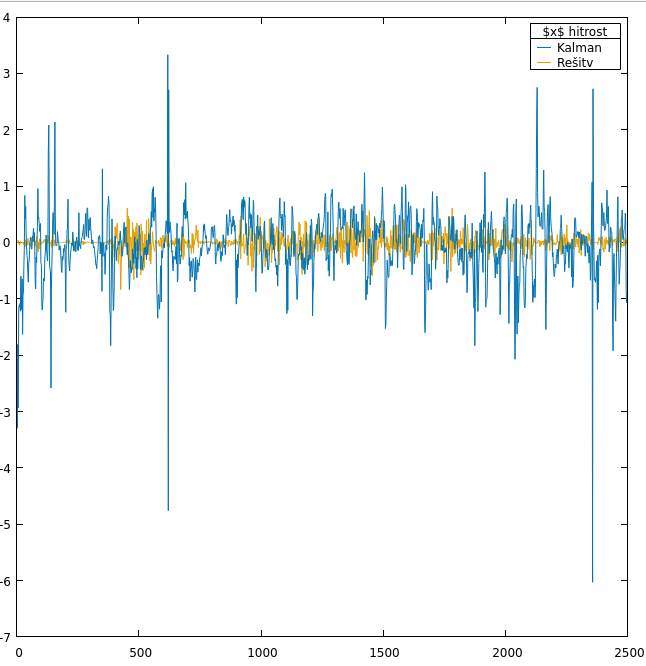
\includegraphics{graf3}}%
    \gplfronttext
  \end{picture}%
\endgroup

    \caption{Poskus povečanja raznolikosti hrane z~omejitvijo količino posameznega živila
    na $200$g.}
    \label{graf3}
\end{figure}

%----------------------------------------------------------------------------------------
%	PROBLEM 2
%----------------------------------------------------------------------------------------

\section{Športna prehrana}
Namesto kalorij minimiziramo vnos maščob in omejimo količino kalorij na $2000$kcal.
Jedilnik tudi na tak način ni zelo raznolik in je s~tega vidika precej podoben tistemu iz 
prejšnjega razdelka~\ref{graf4}.
\begin{figure}    
    % GNUPLOT: LaTeX picture with Postscript
\begingroup
  \makeatletter
  \providecommand\color[2][]{%
    \GenericError{(gnuplot) \space\space\space\@spaces}{%
      Package color not loaded in conjunction with
      terminal option `colourtext'%
    }{See the gnuplot documentation for explanation.%
    }{Either use 'blacktext' in gnuplot or load the package
      color.sty in LaTeX.}%
    \renewcommand\color[2][]{}%
  }%
  \providecommand\includegraphics[2][]{%
    \GenericError{(gnuplot) \space\space\space\@spaces}{%
      Package graphicx or graphics not loaded%
    }{See the gnuplot documentation for explanation.%
    }{The gnuplot epslatex terminal needs graphicx.sty or graphics.sty.}%
    \renewcommand\includegraphics[2][]{}%
  }%
  \providecommand\rotatebox[2]{#2}%
  \@ifundefined{ifGPcolor}{%
    \newif\ifGPcolor
    \GPcolortrue
  }{}%
  \@ifundefined{ifGPblacktext}{%
    \newif\ifGPblacktext
    \GPblacktexttrue
  }{}%
  % define a \g@addto@macro without @ in the name:
  \let\gplgaddtomacro\g@addto@macro
  % define empty templates for all commands taking text:
  \gdef\gplbacktext{}%
  \gdef\gplfronttext{}%
  \makeatother
  \ifGPblacktext
    % no textcolor at all
    \def\colorrgb#1{}%
    \def\colorgray#1{}%
  \else
    % gray or color?
    \ifGPcolor
      \def\colorrgb#1{\color[rgb]{#1}}%
      \def\colorgray#1{\color[gray]{#1}}%
      \expandafter\def\csname LTw\endcsname{\color{white}}%
      \expandafter\def\csname LTb\endcsname{\color{black}}%
      \expandafter\def\csname LTa\endcsname{\color{black}}%
      \expandafter\def\csname LT0\endcsname{\color[rgb]{1,0,0}}%
      \expandafter\def\csname LT1\endcsname{\color[rgb]{0,1,0}}%
      \expandafter\def\csname LT2\endcsname{\color[rgb]{0,0,1}}%
      \expandafter\def\csname LT3\endcsname{\color[rgb]{1,0,1}}%
      \expandafter\def\csname LT4\endcsname{\color[rgb]{0,1,1}}%
      \expandafter\def\csname LT5\endcsname{\color[rgb]{1,1,0}}%
      \expandafter\def\csname LT6\endcsname{\color[rgb]{0,0,0}}%
      \expandafter\def\csname LT7\endcsname{\color[rgb]{1,0.3,0}}%
      \expandafter\def\csname LT8\endcsname{\color[rgb]{0.5,0.5,0.5}}%
    \else
      % gray
      \def\colorrgb#1{\color{black}}%
      \def\colorgray#1{\color[gray]{#1}}%
      \expandafter\def\csname LTw\endcsname{\color{white}}%
      \expandafter\def\csname LTb\endcsname{\color{black}}%
      \expandafter\def\csname LTa\endcsname{\color{black}}%
      \expandafter\def\csname LT0\endcsname{\color{black}}%
      \expandafter\def\csname LT1\endcsname{\color{black}}%
      \expandafter\def\csname LT2\endcsname{\color{black}}%
      \expandafter\def\csname LT3\endcsname{\color{black}}%
      \expandafter\def\csname LT4\endcsname{\color{black}}%
      \expandafter\def\csname LT5\endcsname{\color{black}}%
      \expandafter\def\csname LT6\endcsname{\color{black}}%
      \expandafter\def\csname LT7\endcsname{\color{black}}%
      \expandafter\def\csname LT8\endcsname{\color{black}}%
    \fi
  \fi
    \setlength{\unitlength}{0.0500bp}%
    \ifx\gptboxheight\undefined%
      \newlength{\gptboxheight}%
      \newlength{\gptboxwidth}%
      \newsavebox{\gptboxtext}%
    \fi%
    \setlength{\fboxrule}{0.5pt}%
    \setlength{\fboxsep}{1pt}%
\begin{picture}(7200.00,5040.00)%
    \gplgaddtomacro\gplbacktext{%
      \csname LTb\endcsname%%
      \put(594,220){\makebox(0,0)[r]{\strut{}$-18$}}%
      \csname LTb\endcsname%%
      \put(594,950){\makebox(0,0)[r]{\strut{}$-15$}}%
      \csname LTb\endcsname%%
      \put(594,1680){\makebox(0,0)[r]{\strut{}$-12$}}%
      \csname LTb\endcsname%%
      \put(594,2410){\makebox(0,0)[r]{\strut{}$-9$}}%
      \csname LTb\endcsname%%
      \put(594,3139){\makebox(0,0)[r]{\strut{}$-6$}}%
      \csname LTb\endcsname%%
      \put(594,3869){\makebox(0,0)[r]{\strut{}$-3$}}%
      \csname LTb\endcsname%%
      \put(594,4599){\makebox(0,0)[r]{\strut{}$0$}}%
      \csname LTb\endcsname%%
      \put(726,0){\makebox(0,0){\strut{}}}%
      \csname LTb\endcsname%%
      \put(2245,0){\makebox(0,0){\strut{}}}%
      \csname LTb\endcsname%%
      \put(3765,0){\makebox(0,0){\strut{}}}%
      \csname LTb\endcsname%%
      \put(5284,0){\makebox(0,0){\strut{}}}%
      \csname LTb\endcsname%%
      \put(6803,0){\makebox(0,0){\strut{}}}%
      \put(726,4819){\makebox(0,0){\strut{}$0$}}%
      \put(2245,4819){\makebox(0,0){\strut{}$4$}}%
      \put(3765,4819){\makebox(0,0){\strut{}$8$}}%
      \put(5284,4819){\makebox(0,0){\strut{}$12$}}%
      \put(6803,4819){\makebox(0,0){\strut{}$16$}}%
    }%
    \gplgaddtomacro\gplfronttext{%
      \csname LTb\endcsname%%
      \put(3764,4426){\makebox(0,0){\strut{}poljubni}}%
      \csname LTb\endcsname%%
      \put(3334,3084){\makebox(0,0)[l]{\strut{}$T = 0 $}}%
      \csname LTb\endcsname%%
      \put(3334,3304){\makebox(0,0)[l]{\strut{}$T = 0.1 $}}%
      \csname LTb\endcsname%%
      \put(3334,3524){\makebox(0,0)[l]{\strut{}$T = 0.25 $}}%
      \csname LTb\endcsname%%
      \put(3334,3744){\makebox(0,0)[l]{\strut{}$T = 0.5 $}}%
      \csname LTb\endcsname%%
      \put(3334,3964){\makebox(0,0)[l]{\strut{}$T = 1 $}}%
      \csname LTb\endcsname%%
      \put(3334,4184){\makebox(0,0)[l]{\strut{}$T = 5 $}}%
    }%
    \gplbacktext
    \put(0,0){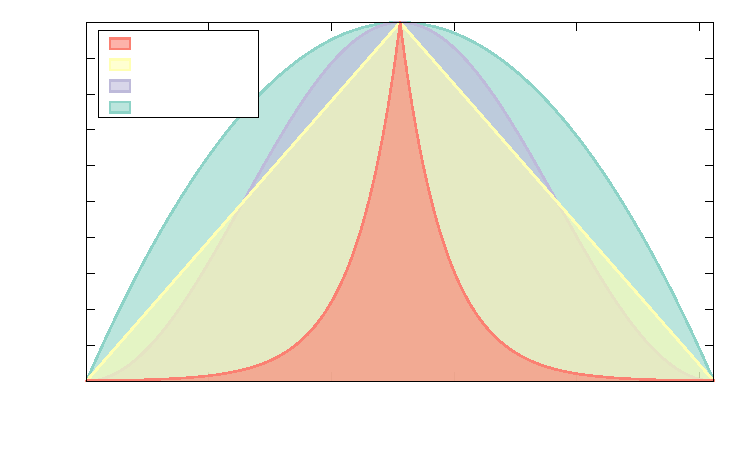
\includegraphics{graf4}}%
    \gplfronttext
  \end{picture}%
\endgroup

    \caption{Minimiziranje maščob, pri dnevnem vnosu $2000$ kcal.}
    \label{graf4}
\end{figure}
Tudi tokrat poskusimo omejiti posamezne količine in z~diagrama~\ref{graf5} vidimo, da
je sedaj jedilnik že precej bolj raznolik, saj smo tako veliko bolj omejili naš 
n-dimenzionalen večkotnik. Pri prikazu je zmanjkalo barv
in se zato ponovijo (v~nasprotni smeri urinega kazalca).
\begin{figure}    
    % GNUPLOT: LaTeX picture with Postscript
\begingroup
  \makeatletter
  \providecommand\color[2][]{%
    \GenericError{(gnuplot) \space\space\space\@spaces}{%
      Package color not loaded in conjunction with
      terminal option `colourtext'%
    }{See the gnuplot documentation for explanation.%
    }{Either use 'blacktext' in gnuplot or load the package
      color.sty in LaTeX.}%
    \renewcommand\color[2][]{}%
  }%
  \providecommand\includegraphics[2][]{%
    \GenericError{(gnuplot) \space\space\space\@spaces}{%
      Package graphicx or graphics not loaded%
    }{See the gnuplot documentation for explanation.%
    }{The gnuplot epslatex terminal needs graphicx.sty or graphics.sty.}%
    \renewcommand\includegraphics[2][]{}%
  }%
  \providecommand\rotatebox[2]{#2}%
  \@ifundefined{ifGPcolor}{%
    \newif\ifGPcolor
    \GPcolortrue
  }{}%
  \@ifundefined{ifGPblacktext}{%
    \newif\ifGPblacktext
    \GPblacktexttrue
  }{}%
  % define a \g@addto@macro without @ in the name:
  \let\gplgaddtomacro\g@addto@macro
  % define empty templates for all commands taking text:
  \gdef\gplbacktext{}%
  \gdef\gplfronttext{}%
  \makeatother
  \ifGPblacktext
    % no textcolor at all
    \def\colorrgb#1{}%
    \def\colorgray#1{}%
  \else
    % gray or color?
    \ifGPcolor
      \def\colorrgb#1{\color[rgb]{#1}}%
      \def\colorgray#1{\color[gray]{#1}}%
      \expandafter\def\csname LTw\endcsname{\color{white}}%
      \expandafter\def\csname LTb\endcsname{\color{black}}%
      \expandafter\def\csname LTa\endcsname{\color{black}}%
      \expandafter\def\csname LT0\endcsname{\color[rgb]{1,0,0}}%
      \expandafter\def\csname LT1\endcsname{\color[rgb]{0,1,0}}%
      \expandafter\def\csname LT2\endcsname{\color[rgb]{0,0,1}}%
      \expandafter\def\csname LT3\endcsname{\color[rgb]{1,0,1}}%
      \expandafter\def\csname LT4\endcsname{\color[rgb]{0,1,1}}%
      \expandafter\def\csname LT5\endcsname{\color[rgb]{1,1,0}}%
      \expandafter\def\csname LT6\endcsname{\color[rgb]{0,0,0}}%
      \expandafter\def\csname LT7\endcsname{\color[rgb]{1,0.3,0}}%
      \expandafter\def\csname LT8\endcsname{\color[rgb]{0.5,0.5,0.5}}%
    \else
      % gray
      \def\colorrgb#1{\color{black}}%
      \def\colorgray#1{\color[gray]{#1}}%
      \expandafter\def\csname LTw\endcsname{\color{white}}%
      \expandafter\def\csname LTb\endcsname{\color{black}}%
      \expandafter\def\csname LTa\endcsname{\color{black}}%
      \expandafter\def\csname LT0\endcsname{\color{black}}%
      \expandafter\def\csname LT1\endcsname{\color{black}}%
      \expandafter\def\csname LT2\endcsname{\color{black}}%
      \expandafter\def\csname LT3\endcsname{\color{black}}%
      \expandafter\def\csname LT4\endcsname{\color{black}}%
      \expandafter\def\csname LT5\endcsname{\color{black}}%
      \expandafter\def\csname LT6\endcsname{\color{black}}%
      \expandafter\def\csname LT7\endcsname{\color{black}}%
      \expandafter\def\csname LT8\endcsname{\color{black}}%
    \fi
  \fi
    \setlength{\unitlength}{0.0500bp}%
    \ifx\gptboxheight\undefined%
      \newlength{\gptboxheight}%
      \newlength{\gptboxwidth}%
      \newsavebox{\gptboxtext}%
    \fi%
    \setlength{\fboxrule}{0.5pt}%
    \setlength{\fboxsep}{1pt}%
\begin{picture}(7200.00,5040.00)%
    \gplgaddtomacro\gplbacktext{%
      \csname LTb\endcsname%%
      \put(594,220){\makebox(0,0)[r]{\strut{}$-18$}}%
      \csname LTb\endcsname%%
      \put(594,950){\makebox(0,0)[r]{\strut{}$-15$}}%
      \csname LTb\endcsname%%
      \put(594,1680){\makebox(0,0)[r]{\strut{}$-12$}}%
      \csname LTb\endcsname%%
      \put(594,2410){\makebox(0,0)[r]{\strut{}$-9$}}%
      \csname LTb\endcsname%%
      \put(594,3139){\makebox(0,0)[r]{\strut{}$-6$}}%
      \csname LTb\endcsname%%
      \put(594,3869){\makebox(0,0)[r]{\strut{}$-3$}}%
      \csname LTb\endcsname%%
      \put(594,4599){\makebox(0,0)[r]{\strut{}$0$}}%
      \csname LTb\endcsname%%
      \put(726,0){\makebox(0,0){\strut{}}}%
      \csname LTb\endcsname%%
      \put(2245,0){\makebox(0,0){\strut{}}}%
      \csname LTb\endcsname%%
      \put(3765,0){\makebox(0,0){\strut{}}}%
      \csname LTb\endcsname%%
      \put(5284,0){\makebox(0,0){\strut{}}}%
      \csname LTb\endcsname%%
      \put(6803,0){\makebox(0,0){\strut{}}}%
      \put(726,4819){\makebox(0,0){\strut{}$0$}}%
      \put(2245,4819){\makebox(0,0){\strut{}$4$}}%
      \put(3765,4819){\makebox(0,0){\strut{}$8$}}%
      \put(5284,4819){\makebox(0,0){\strut{}$12$}}%
      \put(6803,4819){\makebox(0,0){\strut{}$16$}}%
    }%
    \gplgaddtomacro\gplfronttext{%
      \csname LTb\endcsname%%
      \put(3764,4426){\makebox(0,0){\strut{}sosedi}}%
      \csname LTb\endcsname%%
      \put(3334,3084){\makebox(0,0)[l]{\strut{}$T = 0 $}}%
      \csname LTb\endcsname%%
      \put(3334,3304){\makebox(0,0)[l]{\strut{}$T = 0.1 $}}%
      \csname LTb\endcsname%%
      \put(3334,3524){\makebox(0,0)[l]{\strut{}$T = 0.25 $}}%
      \csname LTb\endcsname%%
      \put(3334,3744){\makebox(0,0)[l]{\strut{}$T = 0.5 $}}%
      \csname LTb\endcsname%%
      \put(3334,3964){\makebox(0,0)[l]{\strut{}$T = 1 $}}%
      \csname LTb\endcsname%%
      \put(3334,4184){\makebox(0,0)[l]{\strut{}$T = 5 $}}%
    }%
    \gplbacktext
    \put(0,0){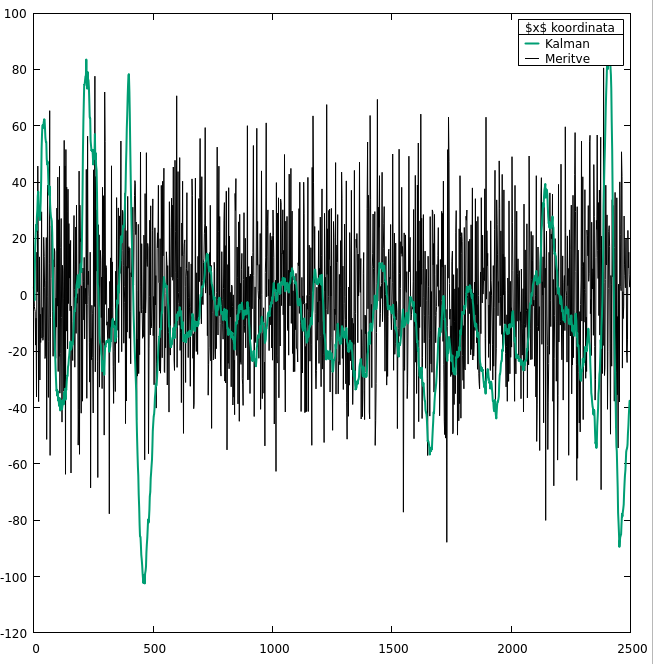
\includegraphics{graf5}}%
    \gplfronttext
  \end{picture}%
\endgroup

    \caption{Minimiziranje maščob, pri dnevnem vnosu $2000$ kcal in omejitvijo posameznih
    živil na $200$g.}
    \label{graf5}
\end{figure}
%----------------------------------------------------------------------------------------
%	PROBLEM 3
%----------------------------------------------------------------------------------------
\section{Varčevanje denarja}
Na~spletni strani priljubljenega trgovskega podjetja lahko poiščemo cene živil in jih
dodamo v~tabelo podatkov. Na podoben način kot pri prejšnjih problemih minimiziramo
ceno dnevnega obroka in dobimo jedilnik na sliki~\ref{graf6} ter spet s~poskusom povečanja
raznolikosti še omejene količine hrane na sliki~\ref{graf7}. Za prvi jedilnik tako
dnevno porabimo $1,61$\euro{} za drugega pa $2,16$\euro{}. Enako sledi še za športni
jedilnik kjer porabi za jedilnik~\ref{graf8} $1,49$\euro{} in za~\ref{gra9} $2,08$\euro{}.
\begin{figure}    
    % GNUPLOT: LaTeX picture with Postscript
\begingroup
  \makeatletter
  \providecommand\color[2][]{%
    \GenericError{(gnuplot) \space\space\space\@spaces}{%
      Package color not loaded in conjunction with
      terminal option `colourtext'%
    }{See the gnuplot documentation for explanation.%
    }{Either use 'blacktext' in gnuplot or load the package
      color.sty in LaTeX.}%
    \renewcommand\color[2][]{}%
  }%
  \providecommand\includegraphics[2][]{%
    \GenericError{(gnuplot) \space\space\space\@spaces}{%
      Package graphicx or graphics not loaded%
    }{See the gnuplot documentation for explanation.%
    }{The gnuplot epslatex terminal needs graphicx.sty or graphics.sty.}%
    \renewcommand\includegraphics[2][]{}%
  }%
  \providecommand\rotatebox[2]{#2}%
  \@ifundefined{ifGPcolor}{%
    \newif\ifGPcolor
    \GPcolortrue
  }{}%
  \@ifundefined{ifGPblacktext}{%
    \newif\ifGPblacktext
    \GPblacktexttrue
  }{}%
  % define a \g@addto@macro without @ in the name:
  \let\gplgaddtomacro\g@addto@macro
  % define empty templates for all commands taking text:
  \gdef\gplbacktext{}%
  \gdef\gplfronttext{}%
  \makeatother
  \ifGPblacktext
    % no textcolor at all
    \def\colorrgb#1{}%
    \def\colorgray#1{}%
  \else
    % gray or color?
    \ifGPcolor
      \def\colorrgb#1{\color[rgb]{#1}}%
      \def\colorgray#1{\color[gray]{#1}}%
      \expandafter\def\csname LTw\endcsname{\color{white}}%
      \expandafter\def\csname LTb\endcsname{\color{black}}%
      \expandafter\def\csname LTa\endcsname{\color{black}}%
      \expandafter\def\csname LT0\endcsname{\color[rgb]{1,0,0}}%
      \expandafter\def\csname LT1\endcsname{\color[rgb]{0,1,0}}%
      \expandafter\def\csname LT2\endcsname{\color[rgb]{0,0,1}}%
      \expandafter\def\csname LT3\endcsname{\color[rgb]{1,0,1}}%
      \expandafter\def\csname LT4\endcsname{\color[rgb]{0,1,1}}%
      \expandafter\def\csname LT5\endcsname{\color[rgb]{1,1,0}}%
      \expandafter\def\csname LT6\endcsname{\color[rgb]{0,0,0}}%
      \expandafter\def\csname LT7\endcsname{\color[rgb]{1,0.3,0}}%
      \expandafter\def\csname LT8\endcsname{\color[rgb]{0.5,0.5,0.5}}%
    \else
      % gray
      \def\colorrgb#1{\color{black}}%
      \def\colorgray#1{\color[gray]{#1}}%
      \expandafter\def\csname LTw\endcsname{\color{white}}%
      \expandafter\def\csname LTb\endcsname{\color{black}}%
      \expandafter\def\csname LTa\endcsname{\color{black}}%
      \expandafter\def\csname LT0\endcsname{\color{black}}%
      \expandafter\def\csname LT1\endcsname{\color{black}}%
      \expandafter\def\csname LT2\endcsname{\color{black}}%
      \expandafter\def\csname LT3\endcsname{\color{black}}%
      \expandafter\def\csname LT4\endcsname{\color{black}}%
      \expandafter\def\csname LT5\endcsname{\color{black}}%
      \expandafter\def\csname LT6\endcsname{\color{black}}%
      \expandafter\def\csname LT7\endcsname{\color{black}}%
      \expandafter\def\csname LT8\endcsname{\color{black}}%
    \fi
  \fi
    \setlength{\unitlength}{0.0500bp}%
    \ifx\gptboxheight\undefined%
      \newlength{\gptboxheight}%
      \newlength{\gptboxwidth}%
      \newsavebox{\gptboxtext}%
    \fi%
    \setlength{\fboxrule}{0.5pt}%
    \setlength{\fboxsep}{1pt}%
\begin{picture}(7200.00,5040.00)%
    \gplgaddtomacro\gplbacktext{%
      \csname LTb\endcsname%%
      \put(462,440){\makebox(0,0)[r]{\strut{}$0$}}%
      \put(462,1316){\makebox(0,0)[r]{\strut{}$5$}}%
      \put(462,2192){\makebox(0,0)[r]{\strut{}$10$}}%
      \put(462,3067){\makebox(0,0)[r]{\strut{}$15$}}%
      \put(462,3943){\makebox(0,0)[r]{\strut{}$20$}}%
      \put(462,4819){\makebox(0,0)[r]{\strut{}$25$}}%
      \put(594,220){\makebox(0,0){\strut{}$0$}}%
      \put(1836,220){\makebox(0,0){\strut{}$2$}}%
      \put(3078,220){\makebox(0,0){\strut{}$4$}}%
      \put(4319,220){\makebox(0,0){\strut{}$6$}}%
      \put(5561,220){\makebox(0,0){\strut{}$8$}}%
      \put(6803,220){\makebox(0,0){\strut{}$10$}}%
    }%
    \gplgaddtomacro\gplfronttext{%
      \csname LTb\endcsname%%
      \put(5086,3216){\makebox(0,0)[l]{\strut{}$ \Delta t = 0.001$}}%
      \csname LTb\endcsname%%
      \put(5086,3436){\makebox(0,0)[l]{\strut{}$ \Delta t = 0.01$}}%
      \csname LTb\endcsname%%
      \put(5086,3656){\makebox(0,0)[l]{\strut{}$ \Delta t = 0.1$}}%
      \csname LTb\endcsname%%
      \put(5086,3876){\makebox(0,0)[l]{\strut{}$ \Delta t = 0.25$}}%
      \csname LTb\endcsname%%
      \put(5086,4096){\makebox(0,0)[l]{\strut{}$ \Delta t = 0.5$}}%
      \csname LTb\endcsname%%
      \put(5086,4316){\makebox(0,0)[l]{\strut{}$ \Delta t = 1$}}%
      \csname LTb\endcsname%%
      \put(5086,4536){\makebox(0,0)[l]{\strut{}$N_0 \mathrm{e}^{-\beta t}$}}%
    }%
    \gplbacktext
    \put(0,0){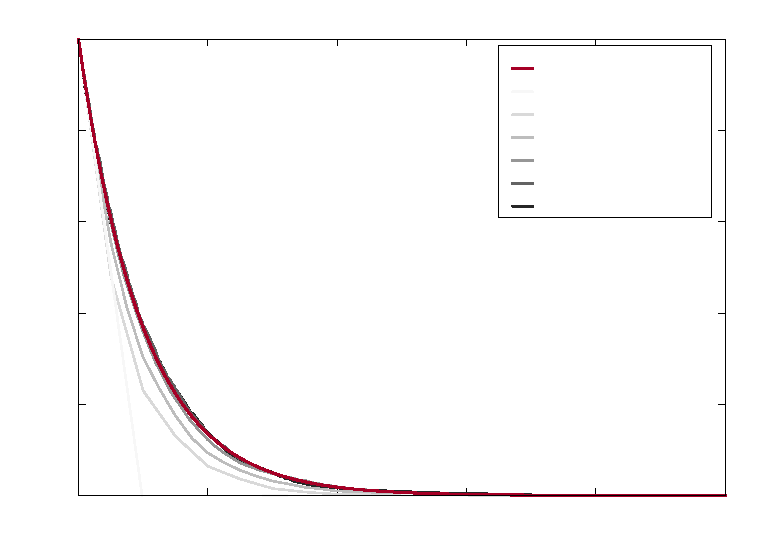
\includegraphics[width={360.00bp},height={252.00bp}]{graf6}}%
    \gplfronttext
  \end{picture}%
\endgroup

    \caption{Minimiziranje cen dnevnih obrokov.}
    \label{graf6}
\end{figure}
\begin{figure}    
    % GNUPLOT: LaTeX picture with Postscript
\begingroup
  \makeatletter
  \providecommand\color[2][]{%
    \GenericError{(gnuplot) \space\space\space\@spaces}{%
      Package color not loaded in conjunction with
      terminal option `colourtext'%
    }{See the gnuplot documentation for explanation.%
    }{Either use 'blacktext' in gnuplot or load the package
      color.sty in LaTeX.}%
    \renewcommand\color[2][]{}%
  }%
  \providecommand\includegraphics[2][]{%
    \GenericError{(gnuplot) \space\space\space\@spaces}{%
      Package graphicx or graphics not loaded%
    }{See the gnuplot documentation for explanation.%
    }{The gnuplot epslatex terminal needs graphicx.sty or graphics.sty.}%
    \renewcommand\includegraphics[2][]{}%
  }%
  \providecommand\rotatebox[2]{#2}%
  \@ifundefined{ifGPcolor}{%
    \newif\ifGPcolor
    \GPcolortrue
  }{}%
  \@ifundefined{ifGPblacktext}{%
    \newif\ifGPblacktext
    \GPblacktexttrue
  }{}%
  % define a \g@addto@macro without @ in the name:
  \let\gplgaddtomacro\g@addto@macro
  % define empty templates for all commands taking text:
  \gdef\gplbacktext{}%
  \gdef\gplfronttext{}%
  \makeatother
  \ifGPblacktext
    % no textcolor at all
    \def\colorrgb#1{}%
    \def\colorgray#1{}%
  \else
    % gray or color?
    \ifGPcolor
      \def\colorrgb#1{\color[rgb]{#1}}%
      \def\colorgray#1{\color[gray]{#1}}%
      \expandafter\def\csname LTw\endcsname{\color{white}}%
      \expandafter\def\csname LTb\endcsname{\color{black}}%
      \expandafter\def\csname LTa\endcsname{\color{black}}%
      \expandafter\def\csname LT0\endcsname{\color[rgb]{1,0,0}}%
      \expandafter\def\csname LT1\endcsname{\color[rgb]{0,1,0}}%
      \expandafter\def\csname LT2\endcsname{\color[rgb]{0,0,1}}%
      \expandafter\def\csname LT3\endcsname{\color[rgb]{1,0,1}}%
      \expandafter\def\csname LT4\endcsname{\color[rgb]{0,1,1}}%
      \expandafter\def\csname LT5\endcsname{\color[rgb]{1,1,0}}%
      \expandafter\def\csname LT6\endcsname{\color[rgb]{0,0,0}}%
      \expandafter\def\csname LT7\endcsname{\color[rgb]{1,0.3,0}}%
      \expandafter\def\csname LT8\endcsname{\color[rgb]{0.5,0.5,0.5}}%
    \else
      % gray
      \def\colorrgb#1{\color{black}}%
      \def\colorgray#1{\color[gray]{#1}}%
      \expandafter\def\csname LTw\endcsname{\color{white}}%
      \expandafter\def\csname LTb\endcsname{\color{black}}%
      \expandafter\def\csname LTa\endcsname{\color{black}}%
      \expandafter\def\csname LT0\endcsname{\color{black}}%
      \expandafter\def\csname LT1\endcsname{\color{black}}%
      \expandafter\def\csname LT2\endcsname{\color{black}}%
      \expandafter\def\csname LT3\endcsname{\color{black}}%
      \expandafter\def\csname LT4\endcsname{\color{black}}%
      \expandafter\def\csname LT5\endcsname{\color{black}}%
      \expandafter\def\csname LT6\endcsname{\color{black}}%
      \expandafter\def\csname LT7\endcsname{\color{black}}%
      \expandafter\def\csname LT8\endcsname{\color{black}}%
    \fi
  \fi
    \setlength{\unitlength}{0.0500bp}%
    \ifx\gptboxheight\undefined%
      \newlength{\gptboxheight}%
      \newlength{\gptboxwidth}%
      \newsavebox{\gptboxtext}%
    \fi%
    \setlength{\fboxrule}{0.5pt}%
    \setlength{\fboxsep}{1pt}%
\begin{picture}(7200.00,5040.00)%
    \gplgaddtomacro\gplbacktext{%
      \csname LTb\endcsname%%
      \put(594,440){\makebox(0,0)[r]{\strut{}$0.1$}}%
      \put(594,1900){\makebox(0,0)[r]{\strut{}$1$}}%
      \put(594,3359){\makebox(0,0)[r]{\strut{}$10$}}%
      \put(594,4819){\makebox(0,0)[r]{\strut{}$100$}}%
      \put(726,220){\makebox(0,0){\strut{}$0$}}%
      \put(1941,220){\makebox(0,0){\strut{}$2$}}%
      \put(3157,220){\makebox(0,0){\strut{}$4$}}%
      \put(4372,220){\makebox(0,0){\strut{}$6$}}%
      \put(5588,220){\makebox(0,0){\strut{}$8$}}%
      \put(6803,220){\makebox(0,0){\strut{}$10$}}%
    }%
    \gplgaddtomacro\gplfronttext{%
      \csname LTb\endcsname%%
      \put(5086,3216){\makebox(0,0)[l]{\strut{}$ \Delta t = 0.001$}}%
      \csname LTb\endcsname%%
      \put(5086,3436){\makebox(0,0)[l]{\strut{}$ \Delta t = 0.01$}}%
      \csname LTb\endcsname%%
      \put(5086,3656){\makebox(0,0)[l]{\strut{}$ \Delta t = 0.1$}}%
      \csname LTb\endcsname%%
      \put(5086,3876){\makebox(0,0)[l]{\strut{}$ \Delta t = 0.25$}}%
      \csname LTb\endcsname%%
      \put(5086,4096){\makebox(0,0)[l]{\strut{}$ \Delta t = 0.5$}}%
      \csname LTb\endcsname%%
      \put(5086,4316){\makebox(0,0)[l]{\strut{}$ \Delta t = 1$}}%
      \csname LTb\endcsname%%
      \put(5086,4536){\makebox(0,0)[l]{\strut{}$N_0 \mathrm{e}^{-\beta t}$}}%
    }%
    \gplbacktext
    \put(0,0){\includegraphics[width={360.00bp},height={252.00bp}]{graf7}}%
    \gplfronttext
  \end{picture}%
\endgroup

    \caption{Minimiziranje cen dnevnih obrokov z~omejitvijo posameznih živil na $200$g.}
    \label{graf7}
\end{figure}
\begin{figure}    
    % GNUPLOT: LaTeX picture with Postscript
\begingroup
  \makeatletter
  \providecommand\color[2][]{%
    \GenericError{(gnuplot) \space\space\space\@spaces}{%
      Package color not loaded in conjunction with
      terminal option `colourtext'%
    }{See the gnuplot documentation for explanation.%
    }{Either use 'blacktext' in gnuplot or load the package
      color.sty in LaTeX.}%
    \renewcommand\color[2][]{}%
  }%
  \providecommand\includegraphics[2][]{%
    \GenericError{(gnuplot) \space\space\space\@spaces}{%
      Package graphicx or graphics not loaded%
    }{See the gnuplot documentation for explanation.%
    }{The gnuplot epslatex terminal needs graphicx.sty or graphics.sty.}%
    \renewcommand\includegraphics[2][]{}%
  }%
  \providecommand\rotatebox[2]{#2}%
  \@ifundefined{ifGPcolor}{%
    \newif\ifGPcolor
    \GPcolortrue
  }{}%
  \@ifundefined{ifGPblacktext}{%
    \newif\ifGPblacktext
    \GPblacktexttrue
  }{}%
  % define a \g@addto@macro without @ in the name:
  \let\gplgaddtomacro\g@addto@macro
  % define empty templates for all commands taking text:
  \gdef\gplbacktext{}%
  \gdef\gplfronttext{}%
  \makeatother
  \ifGPblacktext
    % no textcolor at all
    \def\colorrgb#1{}%
    \def\colorgray#1{}%
  \else
    % gray or color?
    \ifGPcolor
      \def\colorrgb#1{\color[rgb]{#1}}%
      \def\colorgray#1{\color[gray]{#1}}%
      \expandafter\def\csname LTw\endcsname{\color{white}}%
      \expandafter\def\csname LTb\endcsname{\color{black}}%
      \expandafter\def\csname LTa\endcsname{\color{black}}%
      \expandafter\def\csname LT0\endcsname{\color[rgb]{1,0,0}}%
      \expandafter\def\csname LT1\endcsname{\color[rgb]{0,1,0}}%
      \expandafter\def\csname LT2\endcsname{\color[rgb]{0,0,1}}%
      \expandafter\def\csname LT3\endcsname{\color[rgb]{1,0,1}}%
      \expandafter\def\csname LT4\endcsname{\color[rgb]{0,1,1}}%
      \expandafter\def\csname LT5\endcsname{\color[rgb]{1,1,0}}%
      \expandafter\def\csname LT6\endcsname{\color[rgb]{0,0,0}}%
      \expandafter\def\csname LT7\endcsname{\color[rgb]{1,0.3,0}}%
      \expandafter\def\csname LT8\endcsname{\color[rgb]{0.5,0.5,0.5}}%
    \else
      % gray
      \def\colorrgb#1{\color{black}}%
      \def\colorgray#1{\color[gray]{#1}}%
      \expandafter\def\csname LTw\endcsname{\color{white}}%
      \expandafter\def\csname LTb\endcsname{\color{black}}%
      \expandafter\def\csname LTa\endcsname{\color{black}}%
      \expandafter\def\csname LT0\endcsname{\color{black}}%
      \expandafter\def\csname LT1\endcsname{\color{black}}%
      \expandafter\def\csname LT2\endcsname{\color{black}}%
      \expandafter\def\csname LT3\endcsname{\color{black}}%
      \expandafter\def\csname LT4\endcsname{\color{black}}%
      \expandafter\def\csname LT5\endcsname{\color{black}}%
      \expandafter\def\csname LT6\endcsname{\color{black}}%
      \expandafter\def\csname LT7\endcsname{\color{black}}%
      \expandafter\def\csname LT8\endcsname{\color{black}}%
    \fi
  \fi
    \setlength{\unitlength}{0.0500bp}%
    \ifx\gptboxheight\undefined%
      \newlength{\gptboxheight}%
      \newlength{\gptboxwidth}%
      \newsavebox{\gptboxtext}%
    \fi%
    \setlength{\fboxrule}{0.5pt}%
    \setlength{\fboxsep}{1pt}%
\begin{picture}(7200.00,4320.00)%
    \gplgaddtomacro\gplbacktext{%
      \csname LTb\endcsname%%
      \put(504,408){\makebox(0,0)[r]{\strut{}$0$}}%
      \csname LTb\endcsname%%
      \put(504,954){\makebox(0,0)[r]{\strut{}$0.1$}}%
      \csname LTb\endcsname%%
      \put(504,1501){\makebox(0,0)[r]{\strut{}$0.2$}}%
      \csname LTb\endcsname%%
      \put(504,2048){\makebox(0,0)[r]{\strut{}$0.3$}}%
      \csname LTb\endcsname%%
      \put(504,2594){\makebox(0,0)[r]{\strut{}$0.4$}}%
      \csname LTb\endcsname%%
      \put(504,3140){\makebox(0,0)[r]{\strut{}$0.5$}}%
      \csname LTb\endcsname%%
      \put(504,3687){\makebox(0,0)[r]{\strut{}$0.6$}}%
      \csname LTb\endcsname%%
      \put(616,204){\makebox(0,0){\strut{}$0$}}%
      \csname LTb\endcsname%%
      \put(1308,204){\makebox(0,0){\strut{}$1$}}%
      \csname LTb\endcsname%%
      \put(2000,204){\makebox(0,0){\strut{}$2$}}%
      \csname LTb\endcsname%%
      \put(2692,204){\makebox(0,0){\strut{}$3$}}%
      \csname LTb\endcsname%%
      \put(3384,204){\makebox(0,0){\strut{}$4$}}%
      \csname LTb\endcsname%%
      \put(4075,204){\makebox(0,0){\strut{}$5$}}%
      \csname LTb\endcsname%%
      \put(4767,204){\makebox(0,0){\strut{}$6$}}%
      \csname LTb\endcsname%%
      \put(5459,204){\makebox(0,0){\strut{}$7$}}%
      \csname LTb\endcsname%%
      \put(6151,204){\makebox(0,0){\strut{}$8$}}%
      \csname LTb\endcsname%%
      \put(6843,204){\makebox(0,0){\strut{}$9$}}%
    }%
    \gplgaddtomacro\gplfronttext{%
      \csname LTb\endcsname%%
      \put(5163,2382){\makebox(0,0)[l]{\strut{}$ \Delta t = 0.001$}}%
      \csname LTb\endcsname%%
      \put(5163,2586){\makebox(0,0)[l]{\strut{}$ \Delta t = 0.01$}}%
      \csname LTb\endcsname%%
      \put(5163,2790){\makebox(0,0)[l]{\strut{}$ \Delta t = 0.1$}}%
      \csname LTb\endcsname%%
      \put(5163,2994){\makebox(0,0)[l]{\strut{}$ \Delta t = 0.25$}}%
      \csname LTb\endcsname%%
      \put(5163,3198){\makebox(0,0)[l]{\strut{}$ \Delta t = 0.5$}}%
      \csname LTb\endcsname%%
      \put(5163,3402){\makebox(0,0)[l]{\strut{}$ \Delta t = 1$}}%
      \csname LTb\endcsname%%
      \put(3729,3993){\makebox(0,0){\strut{}$N_0 = 25$}}%
    }%
    \gplbacktext
    \put(0,0){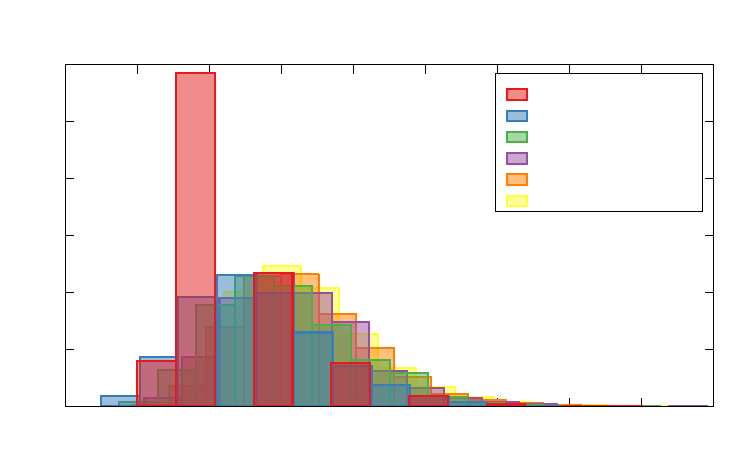
\includegraphics[width={360.00bp},height={216.00bp}]{graf8}}%
    \gplfronttext
  \end{picture}%
\endgroup

    \caption{Minimiziranje cen dnevnih obrokov z~minimalnim vnosom $2000$kcal.}
    \label{graf8}
\end{figure}
\begin{figure}    
    % GNUPLOT: LaTeX picture with Postscript
\begingroup
  \makeatletter
  \providecommand\color[2][]{%
    \GenericError{(gnuplot) \space\space\space\@spaces}{%
      Package color not loaded in conjunction with
      terminal option `colourtext'%
    }{See the gnuplot documentation for explanation.%
    }{Either use 'blacktext' in gnuplot or load the package
      color.sty in LaTeX.}%
    \renewcommand\color[2][]{}%
  }%
  \providecommand\includegraphics[2][]{%
    \GenericError{(gnuplot) \space\space\space\@spaces}{%
      Package graphicx or graphics not loaded%
    }{See the gnuplot documentation for explanation.%
    }{The gnuplot epslatex terminal needs graphicx.sty or graphics.sty.}%
    \renewcommand\includegraphics[2][]{}%
  }%
  \providecommand\rotatebox[2]{#2}%
  \@ifundefined{ifGPcolor}{%
    \newif\ifGPcolor
    \GPcolortrue
  }{}%
  \@ifundefined{ifGPblacktext}{%
    \newif\ifGPblacktext
    \GPblacktexttrue
  }{}%
  % define a \g@addto@macro without @ in the name:
  \let\gplgaddtomacro\g@addto@macro
  % define empty templates for all commands taking text:
  \gdef\gplbacktext{}%
  \gdef\gplfronttext{}%
  \makeatother
  \ifGPblacktext
    % no textcolor at all
    \def\colorrgb#1{}%
    \def\colorgray#1{}%
  \else
    % gray or color?
    \ifGPcolor
      \def\colorrgb#1{\color[rgb]{#1}}%
      \def\colorgray#1{\color[gray]{#1}}%
      \expandafter\def\csname LTw\endcsname{\color{white}}%
      \expandafter\def\csname LTb\endcsname{\color{black}}%
      \expandafter\def\csname LTa\endcsname{\color{black}}%
      \expandafter\def\csname LT0\endcsname{\color[rgb]{1,0,0}}%
      \expandafter\def\csname LT1\endcsname{\color[rgb]{0,1,0}}%
      \expandafter\def\csname LT2\endcsname{\color[rgb]{0,0,1}}%
      \expandafter\def\csname LT3\endcsname{\color[rgb]{1,0,1}}%
      \expandafter\def\csname LT4\endcsname{\color[rgb]{0,1,1}}%
      \expandafter\def\csname LT5\endcsname{\color[rgb]{1,1,0}}%
      \expandafter\def\csname LT6\endcsname{\color[rgb]{0,0,0}}%
      \expandafter\def\csname LT7\endcsname{\color[rgb]{1,0.3,0}}%
      \expandafter\def\csname LT8\endcsname{\color[rgb]{0.5,0.5,0.5}}%
    \else
      % gray
      \def\colorrgb#1{\color{black}}%
      \def\colorgray#1{\color[gray]{#1}}%
      \expandafter\def\csname LTw\endcsname{\color{white}}%
      \expandafter\def\csname LTb\endcsname{\color{black}}%
      \expandafter\def\csname LTa\endcsname{\color{black}}%
      \expandafter\def\csname LT0\endcsname{\color{black}}%
      \expandafter\def\csname LT1\endcsname{\color{black}}%
      \expandafter\def\csname LT2\endcsname{\color{black}}%
      \expandafter\def\csname LT3\endcsname{\color{black}}%
      \expandafter\def\csname LT4\endcsname{\color{black}}%
      \expandafter\def\csname LT5\endcsname{\color{black}}%
      \expandafter\def\csname LT6\endcsname{\color{black}}%
      \expandafter\def\csname LT7\endcsname{\color{black}}%
      \expandafter\def\csname LT8\endcsname{\color{black}}%
    \fi
  \fi
    \setlength{\unitlength}{0.0500bp}%
    \ifx\gptboxheight\undefined%
      \newlength{\gptboxheight}%
      \newlength{\gptboxwidth}%
      \newsavebox{\gptboxtext}%
    \fi%
    \setlength{\fboxrule}{0.5pt}%
    \setlength{\fboxsep}{1pt}%
\begin{picture}(7200.00,5040.00)%
    \gplgaddtomacro\gplbacktext{%
      \csname LTb\endcsname%%
      \put(682,704){\makebox(0,0)[r]{\strut{}$-3$}}%
      \put(682,1292){\makebox(0,0)[r]{\strut{}$-2$}}%
      \put(682,1880){\makebox(0,0)[r]{\strut{}$-1$}}%
      \put(682,2468){\makebox(0,0)[r]{\strut{}$0$}}%
      \put(682,3055){\makebox(0,0)[r]{\strut{}$1$}}%
      \put(682,3643){\makebox(0,0)[r]{\strut{}$2$}}%
      \put(682,4231){\makebox(0,0)[r]{\strut{}$3$}}%
      \put(682,4819){\makebox(0,0)[r]{\strut{}$4$}}%
      \put(814,484){\makebox(0,0){\strut{}$0$}}%
      \put(1984,484){\makebox(0,0){\strut{}$100$}}%
      \put(3153,484){\makebox(0,0){\strut{}$200$}}%
      \put(4323,484){\makebox(0,0){\strut{}$300$}}%
      \put(5493,484){\makebox(0,0){\strut{}$400$}}%
      \put(6663,484){\makebox(0,0){\strut{}$500$}}%
    }%
    \gplgaddtomacro\gplfronttext{%
      \csname LTb\endcsname%%
      \put(209,2761){\rotatebox{-270}{\makebox(0,0){\strut{}$u_i(t)$}}}%
      \put(3808,154){\makebox(0,0){\strut{}$t$}}%
      \csname LTb\endcsname%%
      \put(5879,3986){\makebox(0,0)[l]{\strut{}signal3}}%
      \csname LTb\endcsname%%
      \put(5879,4206){\makebox(0,0)[l]{\strut{}signal2}}%
      \csname LTb\endcsname%%
      \put(5879,4426){\makebox(0,0)[l]{\strut{}signal1}}%
      \csname LTb\endcsname%%
      \put(5879,4646){\makebox(0,0)[l]{\strut{}signal0}}%
    }%
    \gplbacktext
    \put(0,0){\includegraphics[width={360.00bp},height={252.00bp}]{graf9}}%
    \gplfronttext
  \end{picture}%
\endgroup

    \caption{Minimiziranje cen dnevnih obrokov z~minimalnim vnosom $2000$kcal in 
    z~omejitvijo posameznih živil na $200$g.}
    \label{graf9}
\end{figure}

\end{document}
